\documentclass[12pt]{article}
\usepackage[margin=0.7in]{geometry}
\usepackage{amsmath}
\usepackage{hyperref}
\usepackage{graphicx}
\usepackage{float}
\usepackage{caption}
\usepackage{subcaption}
\usepackage{listings}

\title{Numerical analysis: Assignment 11}
\author{Niccolo Zuppichini}
\begin{document}

\maketitle

\section*{Exercise 1}

Show that: \\

\begin{equation}
	\sum_{i=0}^{n-1} w^i = 0 \quad \textrm{for} \; n > 1, \quad \textrm{with} \; 
	w = e^{ \frac{2 \pi i}{n} }
	\label{eq:initial}
\end{equation}

The Eq. \ref{eq:initial} is a geometric serie and its sum converges to: 

\begin{equation}
	\sum_{i=0}^{n-1} w_i = \frac{1 - w^{n}}{1 - w}
	\label{eq:statement}
\end{equation}
 
It suffices to prove that $w^n = 1$. By definition:

\begin{equation}
	w^n = (e^{ \frac{2 \pi i}{n} } )^n = e^{2 \pi i} = cos(2 \pi) + i sin(2 \pi) = 1
	\label{eq:identity}
\end{equation}

By inserting the identity $w^n = 1$ (Eq. \ref{eq:identity}) into Eq. \ref{eq:statement} we obtain:

\begin{equation}
	\sum_{i=0}^{n-1} w_i = \frac{1 - 1}{1 - w} = 0
	\label{eq:result} 
\end{equation}

concluding the proof.

\section*{Exercise 2}

The code has been implemented in \textit{exercise2.py} using Python 2.7. The output of my code are three pictures for iterations $0, 50, 100, ..., 1000$ (Fig. \ref{fig:output}).

\begin{figure}[H]
\centering
\begin{subfigure}{.5\textwidth}
  \centering
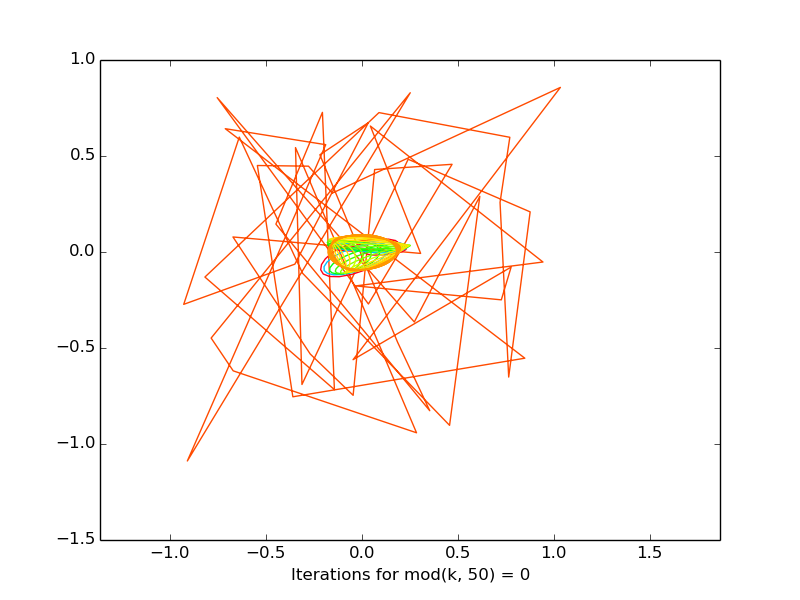
\includegraphics[width = 0.95 \linewidth]{plot1.png}
\end{subfigure}%
\begin{subfigure}{.5\textwidth}
  \centering
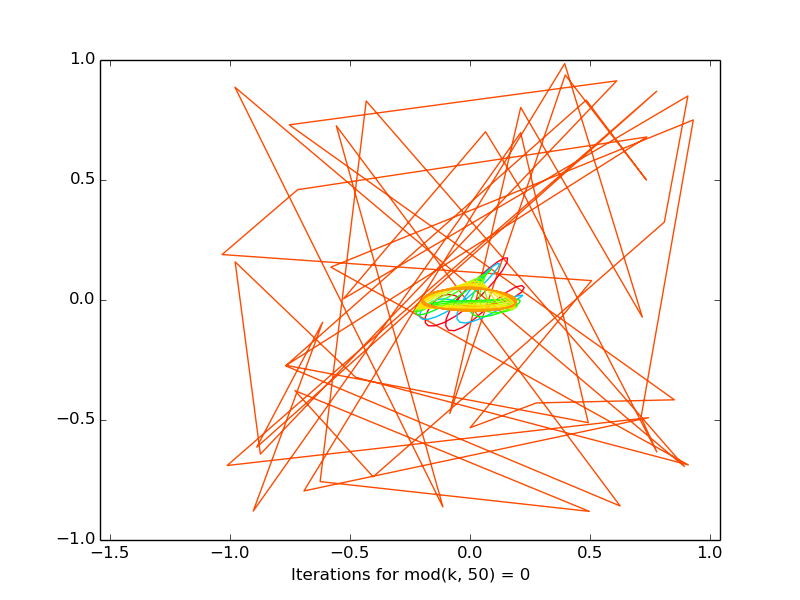
\includegraphics[width = 0.95 \linewidth]{plot2.png}
\end{subfigure}
\label{fig:components}

\begin{subfigure}{.5\textwidth}
  \centering
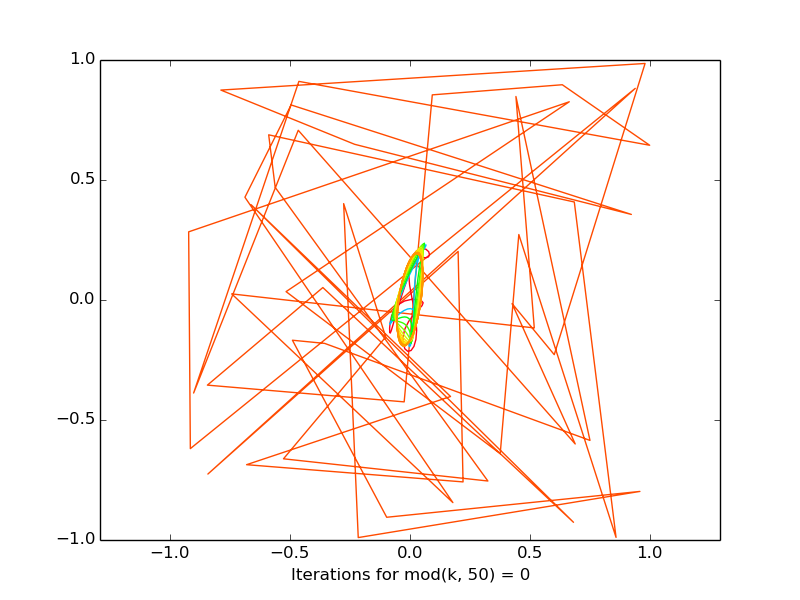
\includegraphics[width = 0.95 \linewidth]{plot3.png}
\end{subfigure}
\caption{Three random polygons and the convergence to their centroids.}
\label{fig:output}
\end{figure}





\end{document}